\resizebox {0.3\columnwidth} {!} {
	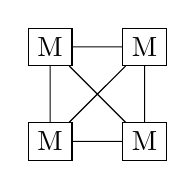
\begin{tikzpicture}[scale=1.2]
		\node[draw] (M1) at (0,0) {M};
		\node[draw] (M2) at (0,1) {M};
		\node[draw] (M3) at (1,0) {M};
		\node[draw] (M4) at (1,1) {M};
		\draw[-] (M1) -- (M2) (M1) -- (M3) (M1) -- (M4)
					(M2) -- (M3) (M2) -- (M4)
					(M3) -- (M4);
	\end{tikzpicture}
}
\subcaption{Miner node network}
\vspace{0.9cm}
\resizebox {0.7\columnwidth} {!} {
	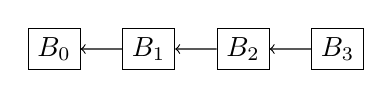
\begin{tikzpicture}	[scale=1.2]
		\node[draw] (B1) at (-1,-1) {$B_0$};
		\node[draw] (B2) at (0,-1) {$B_1$};
		\node[draw] (B3) at (1,-1) {$B_2$};
		\node[draw] (B4) at (2,-1) {$B_3$};

		\draw[->] (B4) -- (B3);
		\draw[->] (B3) -- (B2);
		\draw[->] (B2) -- (B1);
	\end{tikzpicture}
}
\subcaption{Blockchain}